% 03-giai-phap.tex — Chương 3: Nội dung giải pháp

\chapter{Nội dung giải pháp}\label{ch:giaiphap}

\section{Tổng quan dây chuyền sáu bước}

Hệ thống vận hành như một dây chuyền sản xuất: nguyên liệu là dữ liệu thô, thành phẩm là danh sách khách hàng cần chăm sóc
kèm lý do. Mỗi bước có đầu vào, đầu ra và người/đơn vị chịu trách nhiệm rõ ràng.

\begin{figure}[!ht]
\centering
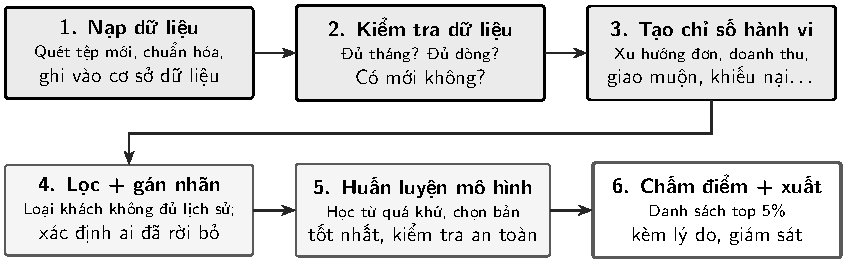
\includegraphics[width=406.2bp]{figures/fig01.pdf}
\caption{Dây chuyền sáu bước từ dữ liệu thô đến danh sách khách hàng ưu tiên}\label{fig:pipeline}
\end{figure}

Hệ thống được chia thành các tầng độc lập, cách chia này giúp khi có sự cố có thể khoanh vùng nhanh, và khi nghiệp vụ thay đổi quy tắc chỉ phải điều chỉnh đúng tầng liên quan.

\section{Phân loại các nhóm khách hàng}

Dựa trên tài liệu nghiệp vụ, khách hàng được chia thành các nhóm có cách xử lý khác nhau:

{\tablefont
\begin{longtable}{@{}L{2.8cm}L{4.6cm}>{\raggedright\arraybackslash}p{7.81cm}@{}}
\caption{Các nhóm khách hàng và cách hệ thống xử lý}\label{tab:nhomkh}\\
\toprule
\hdrrow\hh{Nhóm} & \hh{Định nghĩa nghiệp vụ} & \hh{Cách xử lý hiện nay}\\
\midrule
\endfirsthead
\toprule
\hdrrow\hh{Nhóm} & \hh{Định nghĩa nghiệp vụ} & \hh{Cách xử lý hiện nay}\\
\midrule
\endhead
\bottomrule
\endfoot
\textbf{Rời bỏ} & Tháng tiếp theo không phát sinh đơn, trong khi tháng trước có đơn. & Là một quy tắc chính khi gán nhãn; chỉ khách đang hoạt động và đủ điều kiện mới được chấm điểm.\\
\rowa\textbf{Nguy cơ suy giảm cao} & Số đơn tháng tiếp theo thấp hơn 50\% mức trung bình các tháng trước. & Là tiêu chí chính; mô hình còn học thêm xu hướng doanh thu và mức biến động.\\
\textbf{Khách mới} & Tháng hiện tại là tháng đầu tiên có giao dịch. & Chưa đưa vào dự báo chính; cần theo dõi bằng nhóm riêng.\\
\rowa\textbf{Khách phục hồi} & Từng ngừng, nay phát sinh đơn trở lại. & Có thể tách thành nhóm theo dõi riêng, không trộn vào dữ liệu học.\\
\textbf{Khách mùa vụ} & Phát sinh đơn theo mùa/chu kỳ. & Định hướng phát triển: bổ sung chỉ số mùa vụ để tránh gán nhầm là rời bỏ.\\
\rowa\textbf{Nhóm ưu tiên} & Sản lượng, doanh thu cao. & Đã có bộ lọc theo sản lượng và doanh thu, có thể nâng ngưỡng khi cần.\\
\end{longtable}}
\vspace{4pt}

\section{Lọc ra nhóm khách hàng đủ điều kiện dự báo}\label{sec:loc}

Nếu đưa mọi khách hàng vào, kể cả người chỉ gửi đúng một lần, mô hình sẽ học sai rằng ``ai dùng ngắn hạn cũng là người rời bỏ''.
Điều này làm giảm độ chính xác và khiến danh sách chăm sóc chứa nhiều khách không phù hợp.
Vì vậy hệ thống áp dụng bộ lọc điều kiện giống nhau cho cả lúc học và lúc chấm điểm.

\begin{figure}[!ht]
\centering
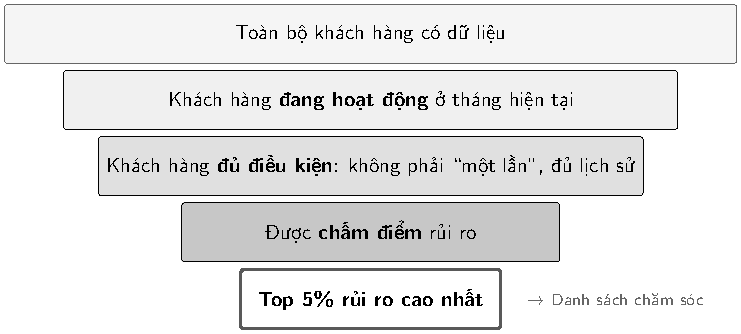
\includegraphics[width=355.9bp]{figures/fig02.pdf}
\caption{Phễu lọc từ toàn bộ khách hàng đến danh sách ưu tiên, sơ đồ minh họa, không thể hiện tỷ lệ thực tế}\label{fig:phau}
\end{figure}

{\tablefont
\begin{longtable}{@{}L{5.0cm}>{\raggedright\arraybackslash}p{10.63cm}@{}}
\caption{Điều kiện lọc khách hàng đủ điều kiện theo cấu hình mặc định}\label{tab:loc}\\
\toprule
\hdrrow\hh{Điều kiện} & \hh{Ý nghĩa}\\
\midrule
\endfirsthead
\toprule
\hdrrow\hh{Điều kiện} & \hh{Ý nghĩa}\\
\midrule
\endhead
\bottomrule
\endfoot
Bật bộ lọc & Áp dụng ở cả bước học và bước chấm điểm, để khách không đủ điều kiện vừa không được ``học'' vừa không xuất hiện trong danh sách.\\
\rowa Tối thiểu 3 tháng phát sinh đơn & Khách phải có ít nhất ba tháng có đơn trong cửa sổ quan sát.\\
Đủ cả cửa sổ khi quan sát ngắn & Nếu chỉ nhìn 3 tháng thì khách phải hoạt động đủ cả 3 tháng.\\
\rowa Tổng số đơn tối thiểu & Loại những khách có sản lượng quá thấp.\\
Tổng doanh thu, giá trị đơn tối thiểu & Có sẵn, hiện đặt ở mức không giới hạn; nghiệp vụ có thể nâng lên để tập trung nhóm giá trị cao.\\
\end{longtable}}
\vspace{4pt}

\section{Biến hành vi thành các chỉ số dễ so sánh}

Mô hình không đọc từng đơn hàng mà đọc một bộ chỉ số hành vi tóm tắt cách khách hàng sử dụng dịch vụ. Chỉ số được chia thành hai nhóm:
nền dài hạn và biến động gần đây. 

{\tablefont
\begin{longtable}{@{}L{3.7cm}>{\raggedright\arraybackslash}p{7.21cm} L{4.3cm}@{}}
\caption{Nhóm chỉ số hành vi chính và ý nghĩa nghiệp vụ}\label{tab:chiso}\\
\toprule
\hdrrow\hh{Nhóm chỉ số} & \hh{Đo điều gì} & \hh{Tín hiệu rủi ro}\\
\midrule
\endfirsthead
\toprule
\hdrrow\hh{Nhóm chỉ số} & \hh{Đo điều gì} & \hh{Tín hiệu rủi ro}\\
\midrule
\endhead
\bottomrule
\endfoot
Quy mô và doanh thu & Tổng đơn, doanh thu, trọng lượng, giá trị trung bình mỗi đơn, trong cửa sổ gần đây & Đơn hoặc doanh thu giảm; giá trị đơn giảm\\
\rowa Xu hướng & Độ dốc tăng/giảm của đơn, doanh thu, điểm hài lòng, khiếu nại theo tháng & Độ dốc âm kéo dài\\
Mức độ biến động & Mức dao động giữa các tháng so với trung bình & Hành vi bất ổn\\
\rowa Mức độ gần đây - tần suất - giá trị & Lần sử dụng gần nhất; mật độ phát sinh; doanh thu nền & Lâu không phát sinh; tần suất giảm\\
Chất lượng dịch vụ & Tỷ lệ giao muộn, hoàn, không chấp nhận, mất; số và đa dạng loại khiếu nại; điểm đơn hàng, điểm hài lòng & Sự cố tăng, hài lòng giảm\\
\rowa Cơ cấu dịch vụ & Số loại dịch vụ dùng, mức độ phụ thuộc một dịch vụ & Thu hẹp dịch vụ sử dụng\\
So với nền dài hạn & Tháng hiện tại so với toàn bộ lịch sử gắn bó của chính khách & Giảm sâu so với ``bình thường'' của khách đó\\
\rowa Thông tin hợp đồng & Khách doanh nghiệp/cá nhân, thời gian gắn bó, địa bàn & Khách mới, gắn bó thấp\\
\end{longtable}}
\vspace{4pt}

\begin{hieunhanh}[Vì sao ``so với nền dài hạn'' quan trọng?]
Một khách hàng gửi 10 đơn mỗi tháng giảm xuống 5 đơn là mất một nửa sản lượng, trong khi khách gửi 10.000 đơn giảm 5 đơn gần như không đáng kể.
Việc so sánh với mức nền của chính từng khách giúp mô hình phân biệt hai trường hợp này.
\end{hieunhanh}

Điểm hài lòng được hệ thống tính từ năm thành phần với trọng số khác nhau (đơn thành công, đơn đúng hạn, chất lượng đơn hàng, độ ổn định,
điểm thưởng/phạt); chi tiết ở Phụ lục~\ref{app:hailong}. Một số trường định danh và trường dễ gây ``rò rỉ'' thông tin tương lai được loại khỏi mô hình để bảo đảm kết quả đáng tin cậy.

\section{Xác định ai là khách hàng rời bỏ: gán nhãn}\label{sec:nhan}

Để mô hình học được, cần có ``đáp án'' cho các tháng đã qua: khách nào thực sự đã rời bỏ. Hệ thống gán nhãn hoàn toàn bằng quy tắc nghiệp vụ, theo nguyên tắc: tại mỗi tháng làm mốc, quan sát hành vi thực tế của khách trong các tháng \emph{tiếp theo}, rồi đối chiếu với các quy tắc dưới đây. Các quy tắc được xây dựng có tham khảo ý kiến của đội chăm sóc khách hàng.

\begin{figure}[!ht]
\centering
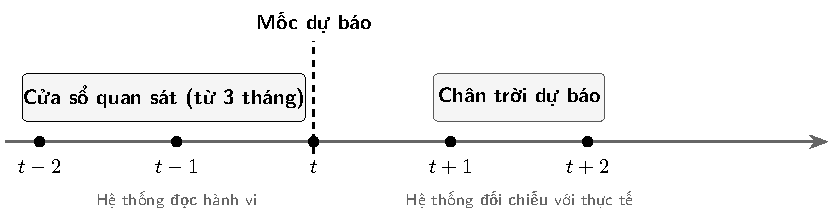
\includegraphics[width=399.8bp]{figures/fig03.pdf}
\caption{Cách chia thời gian khi học: nhìn lịch sử trước mốc, đối chiếu kết quả sau mốc}\label{fig:timeline}
\end{figure}

\subsection{Bốn quy tắc nghiệp vụ gán nhãn}

{\tablefont
\begin{longtable}{@{}L{3.3cm}>{\raggedright\arraybackslash}p{7.91cm} L{4.0cm}@{}}
\caption{Quy tắc gán nhãn khách hàng rời bỏ}\label{tab:nhan}\\
\toprule
\hdrrow\hh{Quy tắc} & \hh{Điều kiện} & \hh{Ý nghĩa}\\
\midrule
\endfirsthead
\toprule
\hdrrow\hh{Quy tắc} & \hh{Điều kiện} & \hh{Ý nghĩa}\\
\midrule
\endhead
\bottomrule
\endfoot
C0 -- Ngừng hẳn & Không còn đơn và không còn doanh thu trong hai tháng sau mốc. & Mất khách hoàn toàn\\
\rowa C1 -- Giảm đơn & Số đơn tương lai giảm hơn 50\% so với mức nền hoặc tháng trước mốc. & Giảm mạnh tần suất gửi\\
C2 -- Giảm doanh thu & Doanh thu tương lai giảm hơn 50\% so với mức nền hoặc tháng trước mốc. & Giảm mạnh giá trị kinh doanh\\
\rowa C3 -- Xu hướng xấu & Doanh thu giảm dần rõ rệt và mức hiện tại dưới 80\% mức nền. & Xu hướng tiêu cực rõ ràng\\
\end{longtable}}
\vspace{4pt}

Ngoài bốn quy tắc trên, hệ thống tính thêm một điểm rủi ro tổng hợp để kiểm soát tỷ lệ khách được gán nhãn rời bỏ cho sát thực tế:
tỷ lệ mục tiêu đặt theo mức mặc định 15\%; vùng ``chưa chắc chắn'' được phân xử bằng quy tắc nghiệp vụ thay vì loại bỏ. Khách hàng chưa đủ dữ liệu sau mốc thì bị loại để không làm tăng giả tạo tỷ lệ rời bỏ.

\section{Mô hình dự báo}

\subsection{Hai lớp mô hình, mỗi lớp một vai trò}

\begin{itemize}
  \item Mô hình cơ sở: là mô hình đơn giản và nhanh dùng để thử nhiều độ dài lịch sử khác nhau và chọn ra vùng cấu hình tốt. Mô hình này dễ giải thích, ổn định, giúp phát hiện sớm sai sót trong nhãn hoặc cách chia dữ liệu và không là mô hình dùng trong vận hành.
  \item Mô hình chính: thuộc nhóm cây quyết định tăng cường, XGBoost là mô hình phổ biến cho dữ liệu dạng bảng; biết xử lý quan hệ phức tạp giữa giảm đơn, doanh thu, khiếu nại, giao muộn và thời gian gắn bó; chịu được dữ liệu thiếu; có cơ chế chống học thuộc lòng và cho phép giải thích lý do.
\end{itemize}

\begin{hieunhanh}[Mô hình dự báo hoạt động thế nào?]
Mô hình giống một nhân viên giàu kinh nghiệm xem lại hàng nghìn khách hàng trong quá khứ: ai rời đi, ai ở lại, và họ đã có những dấu hiệu gì
trước đó. Từ đó, với khách hàng hiện tại, mô hình cho một điểm rủi ro; điểm càng cao thì hành vi càng giống nhóm khách đã rời đi.
\end{hieunhanh}

\subsection{Tinh chỉnh tham số theo hai giai đoạn}

Mô hình chính có nhiều tham số cần chỉnh. Hệ thống làm theo trình tự tiết kiệm công sức nhưng vẫn kỹ lưỡng:

\begin{enumerate}
  \item Thử nhiều độ dài lịch sử bằng mô hình cơ sở để chọn ra các ứng viên tốt nhất.
  \item Huấn luyện mô hình chính cơ bản để xếp hạng ứng viên.
  \item Với ứng viên hàng đầu, tìm kiếm ngẫu nhiên trên vùng rộng để khám phá.
  \item Thu hẹp vùng tốt, rồi dùng phương pháp tối ưu hóa thông minh tinh chỉnh, tự dừng các lần thử kém.
  \item Giữ lại tháng gần nhất làm bài kiểm tra cuối cùng, không dùng trong tinh chỉnh.
\end{enumerate}

\subsection{Kiểm tra theo thời gian, không xáo trộn ngẫu nhiên}

Dữ liệu được chia theo thứ tự thời gian: học từ các tháng cũ, kiểm tra trên các tháng gần hơn, lặp lại nhiều vòng. Giữa phần học và phần kiểm tra có một ``khoảng đệm'' bằng đúng chân trời dự báo để tránh việc mô hình vô tình biết trước tương lai. Ngưỡng cảnh báo trên bài thi cuối kỳ lấy
từ các vòng tinh chỉnh, không tối ưu trực tiếp trên bài thi cuối kỳ.

\begin{luuy}[Vì sao chia theo thời gian?]
Nếu xáo trộn ngẫu nhiên, mô hình có thể được ``học'' từ dữ liệu của tháng sau rồi ``dự báo'' tháng trước đó. Kết quả trên giấy sẽ rất đẹp nhưng không có giá trị khi vận hành thật.
Chia theo thời gian phản ánh đúng cách hệ thống sẽ được dùng.
\end{luuy}

\section{Cách đánh giá chất lượng mô hình}

Mô hình được đánh giá chính bằng điểm F1: đại lượng cân bằng giữa hai điều mà nghiệp vụ quan tâm. Khách hàng rời bỏ chiếm tỷ lệ nhỏ trong tổng thể, nếu chỉ nhìn tỷ lệ đoán đúng chung, một mô hình ``đoán tất cả là không rời bỏ'' vẫn có vẻ chính xác cao nhưng hoàn toàn vô dụng.

{\tablefont
\begin{longtable}{@{}L{3.3cm}>{\raggedright\arraybackslash}p{7.91cm} L{4.0cm}@{}}
\caption{Các thước đo chất lượng mô hình bằng ngôn ngữ nghiệp vụ}\label{tab:metric}\\
\toprule
\hdrrow\hh{Thước đo} & \hh{Câu hỏi nghiệp vụ tương ứng} & \hh{Nếu quá thấp thì sao?}\\
\midrule
\endfirsthead
\toprule
\hdrrow\hh{Thước đo} & \hh{Câu hỏi nghiệp vụ tương ứng} & \hh{Nếu quá thấp thì sao?}\\
\midrule
\endhead
\bottomrule
\endfoot
Độ chính xác cảnh báo & Trong số khách hệ thống cảnh báo, bao nhiêu khách thật sự rời bỏ? & Đội chăm sóc gọi nhầm nhiều\\
\rowa Độ bao phủ & Trong số khách thật sự rời bỏ, hệ thống bắt được bao nhiêu? & Bỏ sót khách rủi ro\\
Điểm F1 & Điểm cân bằng của hai thước đo trên & Mất cân bằng một trong hai\\
\rowa Chất lượng xếp hạng (PR, ROC) & Khách rủi ro cao có được xếp trên khách rủi ro thấp không? & Danh sách ưu tiên kém tin cậy\\
Sai số xác suất & Xác suất mô hình đưa ra có sát thực tế không? & Điểm rủi ro khó tin\\
Ma trận nhầm lẫn & Đếm cảnh báo đúng/sai và bỏ sót để biết mô hình sai theo kiểu nào & Không biết cần chỉnh theo hướng nào\\
\end{longtable}}
\vspace{4pt}

Ngoài các thước đo trên, hệ thống có các rào chắn an toàn: loại mô hình ``cảnh báo tất cả'', loại mô hình có dải điểm quá hẹp, và đối chiếu với các mô hình tham chiếu đơn giản (đoán ngẫu nhiên, đoán hằng số, mô hình hai chỉ số)
để phát hiện bất thường trong nhãn, dữ liệu hoặc cách chia.

\section{Đầu ra của hệ thống}\label{sec:daura}

Mỗi kỳ chấm điểm, hệ thống xuất kết quả theo hai kênh để nghiệp vụ dùng ngay:

{\tablefont
\begin{longtable}{@{}L{4.2cm}>{\raggedright\arraybackslash}p{11.43cm}@{}}
\caption{Đầu ra giao cho nghiệp vụ}\label{tab:daura}\\
\toprule
\hdrrow\hh{Đầu ra} & \hh{Nội dung}\\
\midrule
\endfirsthead
\toprule
\hdrrow\hh{Đầu ra} & \hh{Nội dung}\\
\midrule
\endhead
\bottomrule
\endfoot
Bảng danh sách rủi ro trong cơ sở dữ liệu & Mã khách hàng; kỳ dự báo; các chỉ số gần nhất; xác suất rời bỏ; lý do 1--3; thời điểm cập nhật. Phục vụ truy vấn, báo cáo, kết nối công cụ trực quan.\\
\rowa Tệp CSV xuất định kỳ & Cùng nội dung trên, thêm chi tiết từng lý do. Chia sẻ trực tiếp cho đội chăm sóc.\\
Tệp phân tích giải thích & Mức đóng góp của từng chỉ số vào điểm rủi ro, dùng để kiểm toán mô hình.\\
\end{longtable}}
\vspace{4pt}

\subsection{Phân biệt ba con số dễ nhầm}

Có ba khái niệm nghe gần nhau nhưng khác bản chất; việc phân biệt rõ giúp tránh đọc sai báo cáo:

{\tablefont
\begin{longtable}{@{}L{3.8cm}L{3.6cm}>{\raggedright\arraybackslash}p{7.81cm}@{}}
\caption{Xác suất, thứ hạng và tỷ lệ rời bỏ}\label{tab:phanbiet}\\
\toprule
\hdrrow\hh{Khái niệm} & \hh{Áp dụng cho} & \hh{Ý nghĩa đúng}\\
\midrule
\endfirsthead
\toprule
\hdrrow\hh{Khái niệm} & \hh{Áp dụng cho} & \hh{Ý nghĩa đúng}\\
\midrule
\endhead
\bottomrule
\endfoot
Xác suất rời bỏ & Từng khách hàng & Mô hình ước lượng khả năng khách đó rời bỏ, ví dụ 37\%.\\
\rowa Thứ hạng rủi ro & Từng khách trong tập được chấm & Khách đứng ở vị trí nào so với các khách khác; thứ hạng 97 nghĩa là rủi ro cao hơn 97\% khách còn lại.\\
Tỷ lệ rời bỏ & Một nhóm, một vùng, một tháng & Số khách rời bỏ chia cho số khách đủ điều kiện của nhóm đó.\\
\end{longtable}}
\vspace{4pt}

Danh sách ưu tiên được cắt theo \emph{thứ hạng}: lấy các khách có thứ hạng từ 95 trở lên, tức 5\% khách hàng có rủi ro cao nhất, chứ không phải ``khách có xác suất từ 95\%''.
Cột ``tỷ lệ rời bỏ'' trong bảng kết quả hiện là tên gọi cũ của xác suất theo phần trăm của từng khách; tài liệu bàn giao đã ghi rõ và đề xuất đổi tên cột để tránh hiểu nhầm.

\section{Giải thích lý do rủi ro}\label{sec:lydo}

Điểm rủi ro cao nhưng không có lý do thì đội chăm sóc khó hành động. Hệ thống sử dụng kỹ thuật phân tích mức đóng góp SHAP để xác định chỉ số nào đẩy điểm rủi ro của từng khách lên cao, rồi quy đổi thành tám nhóm lý do nghiệp vụ.
Nếu kỹ thuật này không chạy được, hệ thống tự chuyển sang bộ quy tắc dự phòng để vẫn có lý do.

{\tablefont
\begin{longtable}{@{}L{4.4cm}>{\raggedright\arraybackslash}p{11.23cm}@{}}
\caption{Tám nhóm lý do rủi ro đưa vào danh sách}\label{tab:lydo}\\
\toprule
\hdrrow\hh{Nhóm lý do} & \hh{Nội dung thể hiện cho nghiệp vụ}\\
\midrule
\endfirsthead
\toprule
\hdrrow\hh{Nhóm lý do} & \hh{Nội dung thể hiện cho nghiệp vụ}\\
\midrule
\endhead
\bottomrule
\endfoot
B1 -- Số bưu gửi giảm & Số bưu gửi tháng hiện tại thấp hơn trung bình ba tháng liền trước.\\
\rowa B2 -- Khiếu nại tăng & Số lượng hoặc tỷ lệ khiếu nại tăng.\\
B3 -- Giao muộn tăng & Tỷ lệ hoặc số đơn giao muộn tăng.\\
\rowa B4 -- Đơn không hoàn thành & Đơn hoàn, không chấp nhận, thất lạc tăng.\\
B5 -- Biến động cao & Hành vi gửi hoặc doanh thu dao động mạnh.\\
\rowa B6 -- Giá trị đơn giảm & Doanh thu hoặc giá trị trung bình mỗi đơn giảm theo thời gian.\\
B7 -- Giảm đa dạng dịch vụ & Khách dùng ít loại dịch vụ hơn trước.\\
\rowa B8 -- Khách mới, gắn bó thấp & Khách mới hoặc mức gắn bó thấp.\\
\end{longtable}}
\vspace{4pt}

Trong danh sách xuất ra, mỗi lý do kèm \emph{chỉ số hiện tại}, \emph{mức nền} và \emph{mức thay đổi theo phần trăm}, ví dụ ``số đơn tháng này thấp hơn 60\% so với mức nền''.
Nhờ vậy cán bộ chăm sóc có thể mở đầu cuộc trao đổi bằng chính con số cụ thể của khách hàng.

\begin{figure}[!ht]
\centering
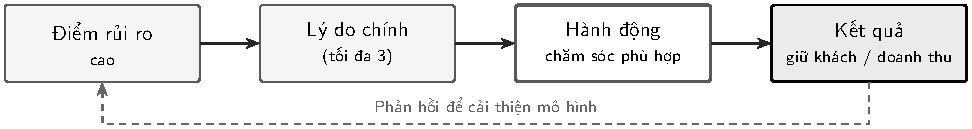
\includegraphics[width=\textwidth]{figures/fig04.pdf}
\caption{Vòng khép kín: từ điểm rủi ro đến hành động và phản hồi}\label{fig:vong}
\end{figure}
